% !TEX program = pdflatex
% !TEX options = -synctex=1 -interaction=nonstopmode -file-line-error "%DOC%"
% 作业模板
\documentclass[UTF8,10pt,a4paper]{article}
\usepackage{ctex}
\newfontfamily\menlo{MONACO.TTF}
\usepackage{amsmath}
\usepackage{diagbox}
\usepackage{float}
\usepackage{listings}
\usepackage{multirow}
\usepackage{tabularx}

\usepackage{url}
\usepackage{xcolor}
\newcommand{\tabincell}[2]{\begin{tabular}{@{}#1@{}}#2\end{tabular}}

\lstset{
    breaklines,                                 % 自动将长的代码行换行排版
    extendedchars=false,                        % 解决代码跨页时,章节标题,页眉等汉字不显示的问题
    backgroundcolor=\color[rgb]{0.96,0.96,0.96},% 背景颜色
    keywordstyle=\color{blue}\bfseries,         % 关键字颜色
    identifierstyle=\color{black},              % 普通标识符颜色
    commentstyle=\color[rgb]{0,0.6,0},          % 注释颜色
    stringstyle=\color[rgb]{0.58,0,0.82},       % 字符串颜色
    showstringspaces=false,                     % 不显示字符串内的空格
    numbers=left,                               % 显示行号
    numberstyle=\tiny\menlo,                    % 设置数字字体
    basicstyle=\small\menlo,                    % 设置基本字体
    captionpos=t,                               % title在上方(在bottom即为b)
    frame=single,                               % 设置代码框形式
    rulecolor=\color[rgb]{0.8,0.8,0.8},         % 设置代码框颜色
}  

\usepackage{pythonhighlight}
\usepackage{listings}
\usepackage{xcolor}
\usepackage{graphicx}
\usepackage[a4paper,left=2cm,right=2cm,top=2cm,bottom=2cm]{geometry}
\usepackage{fancyhdr}
% \catcode`\。=\active
% \newcommand{。}{.}
\newcommand{\CourseName}{操作系统(Operating System)}
\newcommand{\CourseCode}{CS307 \& CS356}
\newcommand{\Semester}{2020-2021学年第二学期}
\newcommand{\ProjectName} {\Huge{Project 8}} 
\newcommand{\StudentName}{刘涵之}
\newcommand{\StudentID}{519021910102}
\usepackage[vmargin=1in,hmargin=.5in]{geometry}
\usepackage{fancyhdr}
\usepackage{lastpage}
\usepackage{calc}
\pagestyle{fancy}
\fancyhf{}
\fancyhead[L]{\CourseName}
\fancyhead[C]{\ProjectName}
\fancyhead[R]{\StudentName}
\fancyfoot[R]{\thepage\ / \pageref{LastPage}}
\setlength\headheight{12pt}
\fancypagestyle{FirstPageStyle}{
    \fancyhf{}
    \fancyhead[L]{\CourseName\\
        \CourseCode\\
        \Semester}
    \fancyhead[C]{\large\bfseries\ProjectName \\}
    \fancyhead[R]{Name: \makebox[\widthof{\StudentID}][s]{\StudentName}\\
        ID : \StudentID\\
        }
    \fancyfoot[R]{\thepage\ / \pageref{LastPage}}
    \setlength\headheight{36pt}
}
\usepackage{amsmath,amssymb,amsthm,bm}
\allowdisplaybreaks[4]
\newtheoremstyle{Problem}
{}
{}
{}
{}
{\bfseries}
{.}
{ }
{第\thmnumber{ #2}\thmname{ #1}\thmnote{ (#3)} 得分: \underline{\qquad\qquad}}
\theoremstyle{Problem}
\newtheorem{prob}{题}
\newtheoremstyle{Solution}
{}
{}
{}
{}
{\bfseries}
{:}
{ }
{\thmname{#1}}
\makeatletter
\def\@endtheorem{\qed\endtrivlist\@endpefalse}
\makeatother
\theoremstyle{Solution}
\newtheorem*{sol}{解}
\title{Project 8: Designing a Virtual Memory Manager}
\date{}
% \usepackage{graphicx}
\begin{document}
\maketitle
\thispagestyle{FirstPageStyle}




This project consists of writing a program that translates logical to physical addresses for a virtual address space of size $2^{16} = 65536$ bytes. The program will read from a file containing logical address and, using a TLB and a page table, will translate each logical address to its corresponding physical address and output the value of the byte stored at the translated physical address. It requires us to use simulation to understand the steps involved in translating logical address to physical address, and this will include resolving page faults using demand paging, managing a TLB, and implementing a page-replacement algorithm.

The program will read a file containing several 32-bit integer numbers that represent logical addresses. However, the 16-bit addresses is the only thing that needs to be concerned, so we must mask the rightmost 16 bits of each logical addresses. These 16 bits are divided into an 8-bit page number and an 8-bit page offset. Hence, the addresses are structured as shown as:
\begin{figure}[htbp]
  \centering
  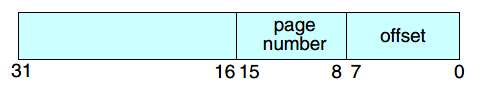
\includegraphics[width=3in]{pic0.png}
\end{figure}

Other specifics includes the following:
\begin{itemize}
  \item $2^8$ entries in the page table;
  \item Page size of $2^8$ bytes;
  \item $16$ entries in the TLB;
  \item Frame size of $2^8$ bytes;
  \item $256$ frames;
  \item Physical memory of $65536$ bytes ($256$ frames $\times$ $256$-byte frame size).
\end{itemize}

The program is to output the following values:
\begin{itemize}
\item The logical address being translated (the integer value being read from \texttt{addresses.txt}).
\item The corresponding physical address (what your program translates the logical address to).
\item The signed byte value stored in physical memory at the translated physical address.
\end{itemize}

We also provide the file \texttt{correct.txt}, which contains the correct output values for the file \texttt{addresses.txt}. You should use this file to determine if the program is correctly translating logical to physical addresses.

After completion, the program is to report the following statistics:
\begin{itemize}
  \item Page-fault rate - The percentage of address references that resulted in page faults.
  \item TLB hit rate - The percentage of address references that were resolved in the TLB.
\end{itemize}

Since the logical addresses in \texttt{addresses.txt} were generated randomly and do not reflect any memory access locality, do not expect to have a high TLB hit rate.

Then use a smaller physical address space with 128 page frames rather than 256. This change will require modifying your program so that it keeps track of free page frames as well as implementing a page-replacement policy using either FIFO or LRU (Section 10.4) to resolve page faults when there is no free memory.



\textbf{Design:} My design for this task is:
\begin{itemize}
    \item All the replacement (memory and TLB) is implemented with LRU algorithm.
    \item \textbf{swap\_page\_in()} function will first search for the empty frame. If there is no empty frame, LRU algorithm will be used to find a victim to swap. The victim will be deleted from TLB using \textbf{delete\_TLB()} function.
    \item For translating a virtual address to a physical one, the program will first look up TLB using \textbf{get\_frame\_TLB()} function. If TLB miss, it will look up \texttt{page\_table} with \texttt{page\_table\_inmem}. If page table miss, it will swap the page in from \texttt{backing\_store} using \textbf{swap\_page\_in()} function.
\end{itemize}


The implementation of the virtual memory manager (\texttt{vmm.c}) is shown as follows.
\begin{lstlisting}[language = c]
#include <stdio.h>
#include <stdlib.h>
#include <string.h>

#define PAGE_NUM 256
#define PAGE_SIZE 256
#define FRAME_NUM 256
#define FRAME_SIZE 256
#define TLB_SIZE 16

int get_frame_TLB(int page_number);
void TLB_update(int page_number, int frame_number);
void delete_TLB(int page_number, int frame_number);

char memory[FRAME_NUM * FRAME_SIZE];

FILE *backing_store;
int total = 0, page_fault = 0, tlb_hit = 0;

int page_table[PAGE_NUM], page_table_inmem[PAGE_NUM];
int frame_count[FRAME_NUM];

void swap_page_out(int frame_number) {
    int page_number = -1;
    
	for (int i = 0; i < PAGE_NUM; i++) {
		if(page_table_inmem[i] > 0 && page_table[i] == frame_number) {
			page_number = i;
			break;
		}
    }
    if (page_number == -1) {
        for (int i = 0; i < PAGE_NUM; i++) {
		
        printf("%d, %d \n", page_table_inmem[i], page_table[i]);
    }
		fprintf(stderr, "[Err] Unexpectedddd Error!\n");
        
		exit(1);
	}
    page_table_inmem[page_number] = 0;

    //TLB delete
    delete_TLB(page_number, frame_number);

    return;
}

int swap_page_in(int page_number) {
    char buf[FRAME_SIZE];
    fseek(backing_store, page_number * FRAME_SIZE, 0);
    fread(buf, sizeof(char), FRAME_SIZE, backing_store);

    int target = -1;
    for (int i = 0; i < FRAME_NUM; i++) {
        if (frame_count[i] == 0) {
            target = i;
            break;
        }
    }
    if (target == -1) {
        for (int i = 0; i < FRAME_NUM; i ++) {
            if (frame_count[i] == FRAME_NUM) {
                target = i;
                break;
            }
        }
        swap_page_out(target);
    }
    for (int i = 0; i < FRAME_SIZE; ++ i) memory[target * FRAME_SIZE + i] = buf[i];
	for (int i = 0; i < FRAME_NUM; ++ i) if (frame_count[i] > 0) frame_count[i]++;
	frame_count[target] = 1;
	return target;
}


int get_val(int frame_number, int offset) {
    int val = (int)memory[frame_number * FRAME_SIZE + offset];

    for (int i = 0; i < FRAME_NUM; ++ i) {
        if (frame_count[i] != 0 && frame_count[i] < frame_count[frame_number])
			frame_count[i]++;
    }
    frame_count[frame_number] = 1;

    return val;
}

int get_frame(int page_number) {

    // TLB
    int tlb_frame = get_frame_TLB(page_number);
    if (tlb_frame != -1) return tlb_frame;

    if (page_table_inmem[page_number] > 0) {

        // TLB
        TLB_update(page_number, page_table[page_number]);

		return page_table[page_number];
	} else {
		page_fault++;
		page_table[page_number] = swap_page_in(page_number);
		page_table_inmem[page_number] = 1;

        // TLB
        TLB_update(page_number, page_table[page_number]);
		return page_table[page_number];
	}
    return -1;
}


// TLB

int TLB_list[TLB_SIZE][2]; // 0 -> page; 1 -> frame
int TLB_count[TLB_SIZE];

int get_frame_TLB(int page_number) {
    int frame = -1, loc = -1;
    for (int i = 0; i < TLB_SIZE; ++ i)
		if (TLB_count[i] != 0 && TLB_list[i][0] == page_number) {
			frame = TLB_list[i][1];
            loc = i;
			break;
		}

    if (frame == -1) return -1; // TLB miss

    tlb_hit++;
    for (int i = 0; i < TLB_SIZE; i++)
        if (TLB_count[i] != 0 && TLB_count[i] < TLB_count[loc]) {
			TLB_count[i]++;
        }
    TLB_count[loc] = 1;

    return frame;
}

void TLB_update(int page_number, int frame_number) {
    int loc = -1;
	for (int i = 0; i < TLB_SIZE; i++)
		if(TLB_count[i] == 0) {
			loc = i;
			break;
		}
	if (loc == -1) {
		for (int i = 0; i < TLB_SIZE; i++)
			if(TLB_count[i] == TLB_SIZE) {
				loc = i;
				break;
			}
	}

    for (int i = 0; i < TLB_SIZE; i++)
		if (TLB_count[i] > 0) TLB_count[i] += 1;

	TLB_count[loc] = 1;
    TLB_list[loc][0] = page_number;
    TLB_list[loc][1] = frame_number;
    return;
}

void delete_TLB(int page_number, int frame_number) {
    int loc = -1;
	for (int i = 0; i < TLB_SIZE; ++ i)
		if(TLB_count[i] == 0) {
			loc = i;
			break;
		}
	if (loc == -1) return; // not find, no need to delete

    for (int i = 0; i < TLB_SIZE; ++ i)
		if (TLB_count[i] > TLB_count[loc]) TLB_count[i] -= 1;

	TLB_count[loc] = 0;
}


int main(int argc, char *argv[]) {
    if (argc != 2) {
        fprintf(stderr, "[Error] Unexpected input!\n");
		return 1;
    }

    backing_store = fopen("BACKING_STORE.bin", "r");

    for (int i = 0; i < PAGE_NUM; i++) {
        page_table[i] = 0;
        page_table_inmem[i] = 0;
    }
    for (int i = 0; i < FRAME_NUM; i++) {
        frame_count[i] = 0;
    }
    for (int i = 0; i < TLB_SIZE; i++) {
        TLB_list[i][0] = 0;
        TLB_list[i][1] = 0;
        TLB_count[i] = 0;
    }

	FILE *stream_in = fopen(argv[1], "r");
	FILE *stream_out = fopen("output.txt", "w");

    int virtual_addr;
    int page_number, offset, frame_number, val;

    while(~fscanf(stream_in, "%d", &virtual_addr)) {
        total += 1;

        virtual_addr = virtual_addr & 0x0000ffff;
        page_number = (virtual_addr >> 8) & 0x000000ff;
		offset = virtual_addr & 0x000000ff;

        frame_number = get_frame(page_number);
        val = get_val(frame_number, offset);

        fprintf(stream_out, "Virtual address: %d Physical address: %d Value: %d\n", virtual_addr, (frame_number << 8) + offset, val);
    }
    fprintf(stdout, "TLB hit rate: %.2f%%      Page fault rate: %.2f%%\n", 100.0 * tlb_hit / total, 100.0 * page_fault / total);

    fclose(stream_in);
    fclose(stream_out);
    
    return 0;
}
\end{lstlisting}


To check the result, i also implement a checker program (\texttt{judge.c}), the main function of it is to compare the value of the answer and the output. If the output is correct, this program will print \textbf{All correct!}, otherwise, it will print \textbf{Wrong answer!}. The code of \texttt{judge.c} is shown as follow.

\begin{lstlisting}[language = c]
#include <stdio.h>
#include <stdlib.h>
#include <string.h>

int main() {
	FILE *stream_ans = fopen("output.txt", "r");
	FILE *stream_std = fopen("correct.txt", "r");
    
    int a, b, c;
    int ac = 0; // 0 => ac; 1 => wrong

    while(~fscanf(stream_ans, "Virtual address: %d Physical address: %d Value: %d\n", &a, &b, &c)) {
        int d, e, f;
        if (fscanf(stream_std, "Virtual address: %d Physical address: %d Value: %d\n", &d, &e, &f) == EOF) {
            printf("File length not match!\n");
			ac = 1;
			break;
        }
        if (c != f) {
            printf("Wrong answer!\n");
			ac = 1;
			break;
        }
    }
    
    if (ac == 0) printf("All correct!\n");

    fclose(stream_ans);
    fclose(stream_std);

    return 0;
}
\end{lstlisting}


Makefile for this task is shown as below:
\begin{lstlisting}
CC=gcc
CFLAGS=-Wall

all: vmm.o judge.o
	$(CC) $(CFLAGS) -o vmm vmm.o
	$(CC) $(CFLAGS) -o judge judge.o

vmm.o: vmm.c
	$(CC) $(CFLAGS) -c vmm.c

judge.o: judge.c
	$(CC) $(CFLAGS) -c judge.c

clean:
	rm -rf *.o
	rm -rf vmm
	rm -rf judge
\end{lstlisting}


When the \textbf{FRAME\_NUM} is 128, the execution result of the virtual memory manager is shown as follows:
\begin{figure}[H]
    \centering
    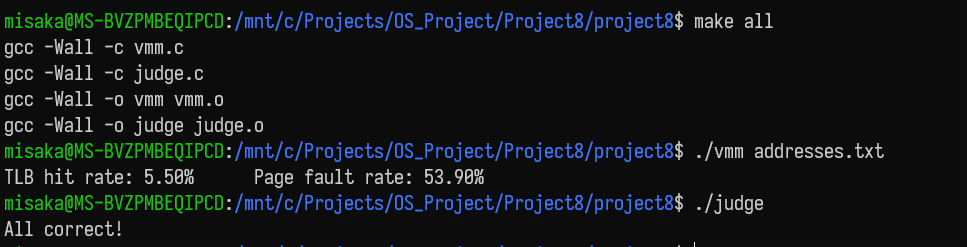
\includegraphics[width=400pt]{1.png}
    \caption{Designing a Virtual Memory Manager (frame number is 128)}
    \label{3}
\end{figure}

When the \textbf{FRAME\_NUM} is 256, the execution result of the virtual memory manager is shown as follows. The page fault rate is dropped.
\begin{figure}[H]
    \centering
    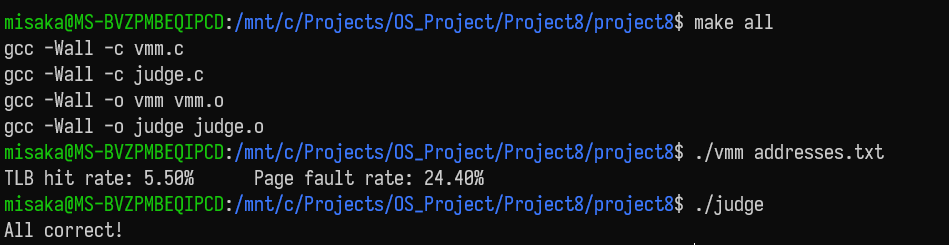
\includegraphics[width=400pt]{2.png}
    \caption{Designing a Virtual Memory Manager (frame number is 256)}
    \label{3}
\end{figure}

\end{document}